\documentclass{article}
\usepackage[utf8]{inputenc}
\usepackage{biblatex}
\usepackage{graphicx}
\usepackage{hyperref}
\addbibresource{references.bib}

\title{Inferential Methods for Protein Folding}
\author{Eric He}
\date{November 2019}

\begin{document}

\maketitle

\section*{Abstract}
The problem of protein folding is centered around understanding how the chain of amino acids comprising a protein folds into its stable, low-energy conformation. Though the laws of physics which govern the process are well-defined, naively using them to simulate folding is computationally intractable. As a result, the protein folding field makes heavy use of statistical methods to infer the structures of unknown proteins based on their similarities to known structures. 

This paper considers the protein folding problem from the inferential perspective. We identify the disparate sources of data which yield information about protein structure, and discuss inferential methods designed to mine that data. The methods covered are:

\begin{itemize}
    \item Bayesian scoring for deriving empirical, "knowledge-based" energy functions which are easier to minimize than the true thermodynamic energy
    \item Monte Carlo methods, such as simulated annealing, stochastic tunneling, and parallel tempering for optimizing energy functions
    \item Some uses of probabilistic graphical models for analysis and inference, namely:
    \begin{itemize}
        \item Markov State Models and Variational Auto-Encoders for aggregating data from protein folding simulations
        \item Markov Random Fields for modeling protein structures
        \item Hidden Markov Models for inferring evolutionary relationships between different amino acid sequences
    \end{itemize}
\end{itemize}

\newpage
\tableofcontents
\newpage

\section{A brief introduction to the protein folding problem}

\begin{figure}
  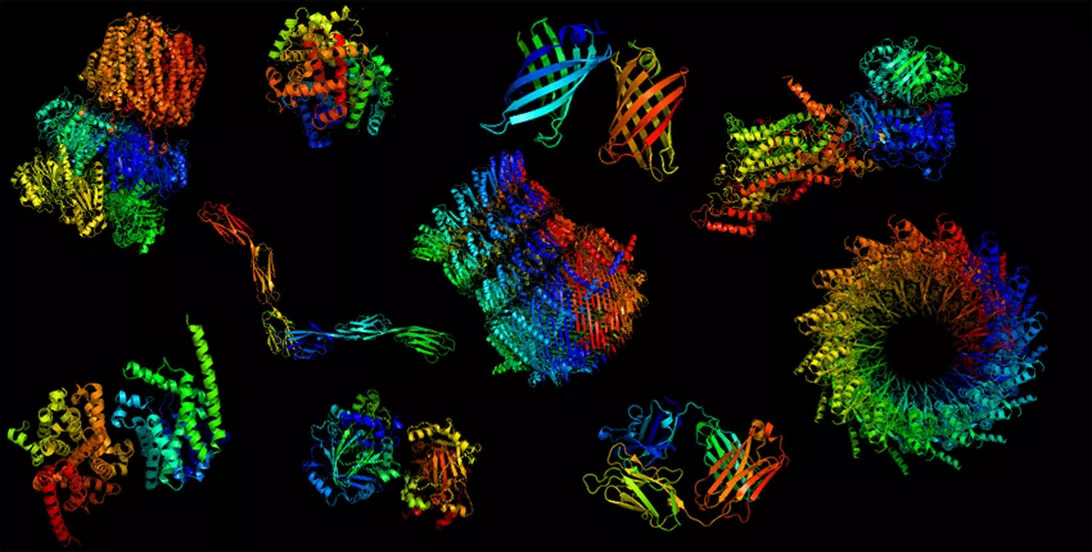
\includegraphics[width=\linewidth]{images/protein_folds.jpg}
  \caption{Examples of computer-generated protein folds by Mohammed Al-Quraishi}
  \label{fig:protein_folds}
\end{figure}

\subsection{The importance of protein folding}
Proteins govern nearly all biological processes, such as metabolizing food, transporting molecules, or providing structure to cells. A protein is created as a sequence of amino acid polymers, which \textit{folds} into a three-dimensional structure or \textbf{conformation} according to the physics of the amino acids comprising them and external forces such as water molecules or other proteins. For the vast majority of proteins, there is only one unique shape which the protein settles into, termed the \textbf{native conformation} or \textbf{native state}.

The native conformation determines a protein's ability to form chemical bonds with other molecules. In turn, a protein's chemical bonding properties determines its ability to perform its desired function; thus, it is commonly said that a protein's structure informs its function. The practical benefits of understanding a protein's native state include, but are not limited to:

\begin{itemize}
    \item modeling the dynamics of a protein's properties under mutations or misfoldings, especially in relation to diseases caused by malfunctioning proteins
    \item discovering drugs which allow us to control the activation or deactivation of target proteins
    \item identifying and tracing a protein's function through the course of its evolutionary history
\end{itemize}

Unfortunately, the minuscule size of proteins make it extremely difficult to map their structures. The only information of most known proteins are their amino acid sequences, derived from genomics data. Filling this gap is the goal of the protein folding problem. From a practical perspective, a mapping between a protein's sequence data and its corresponding structure would link what is known about a protein and what is needed to be known in order to usefully work with it. But more broadly, understanding protein structure provides the theoretical scaffolding needed to analyze biological systems as an emergent product of their underlying components.

\begin{figure}[ht]
  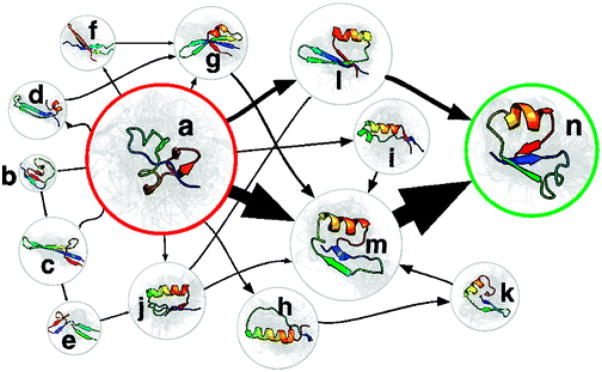
\includegraphics[width=\linewidth]{images/folding_pathways.jpg}
  \caption{Different probable states of a protein fold derived by learning a Markov State Model on Molecular Dynamics simulations in \cite{pande2010}}
  \label{fig:folding_pathways}
\end{figure}

\subsection{Physics underlying protein folding}
The protein folding process is governed entirely by physical laws. The primary ones are:

\begin{enumerate}
    \item The formation of hydrogen bonds between an amino acid residue with other residues in the chain, or the surrounding solvent
    \item van der Waals forces which attract or repel nearby atoms based on their electrostatic charges
    \item Chemical affinities towards the solvent, e.g. hydrophobia of certain molecules to water
\end{enumerate}

Many of the above forces are functions of temperature and acidity. Moreover, the presence of salts, folding catalysts, or \textit{molecular chaperones} can regulate the environment in which the protein folds.

Each of these forces push the amino acid chain towards conformations that lower the \textbf{Gibbs free energy}. The native conformation is typically attained when the free energy is globally minimized, but sometimes proteins can be trapped in a conformation which attains only a local energy minimum. Having proteins \textit{misfold} in such a manner is a known or suspected cause of many diseases such as Alzheimer's or Huntington's.

The vast majority of proteins fold at speeds on the order of nanoseconds to hundreds of milliseconds. Though quick on human timescales, this speed belies the complexity of simulating the process.

\section{Using Molecular Dynamics to simulate protein folding}
Since all physical laws governing protein folding are well-understood, computers can be used to simulate the protein folding process; this field is called \textbf{molecular dynamics} or \textbf{MD}. Unfortunately, simulations of the protein folding process require a tremendous amount of computing power to simulate the folding dynamics of even a single protein. 

\subsection{The computational difficulties of MD simulations}
The primary bottlenecks are the number of particle interactions involved and the amount of time steps to take. Though proteins fold in milliseconds ($10^{-3}$ seconds), simulations take timesteps on the order of femtoseconds ($10^{-15}$), requiring a quadrillion iterations to simulate a full second of folding \cite{md}. For each iteration, all interactions between atoms must be computed. This includes atoms belonging to the enveloping solvent, usually water molecules, which can be more numerous than the protein itself.

To sacrifice some accuracy in order to cut computational cost, MD simulations make various simplifications. \cite{md} gives some examples:

\begin{itemize}
    \item Electrostatic forces are simulated as point charges which might ignore effects such as the electric dipole moment.
    \item Stretching and bending of chemical bonds are modeled using harmonic functions instead of more accurate ones which model anharmonicity.
    \item Water molecules serving as solvent might be modeled as rigid or having a uniform temperature, or modeled only implicitly as a force field exerting random forces on the protein.
\end{itemize} 

\begin{figure}[ht]
  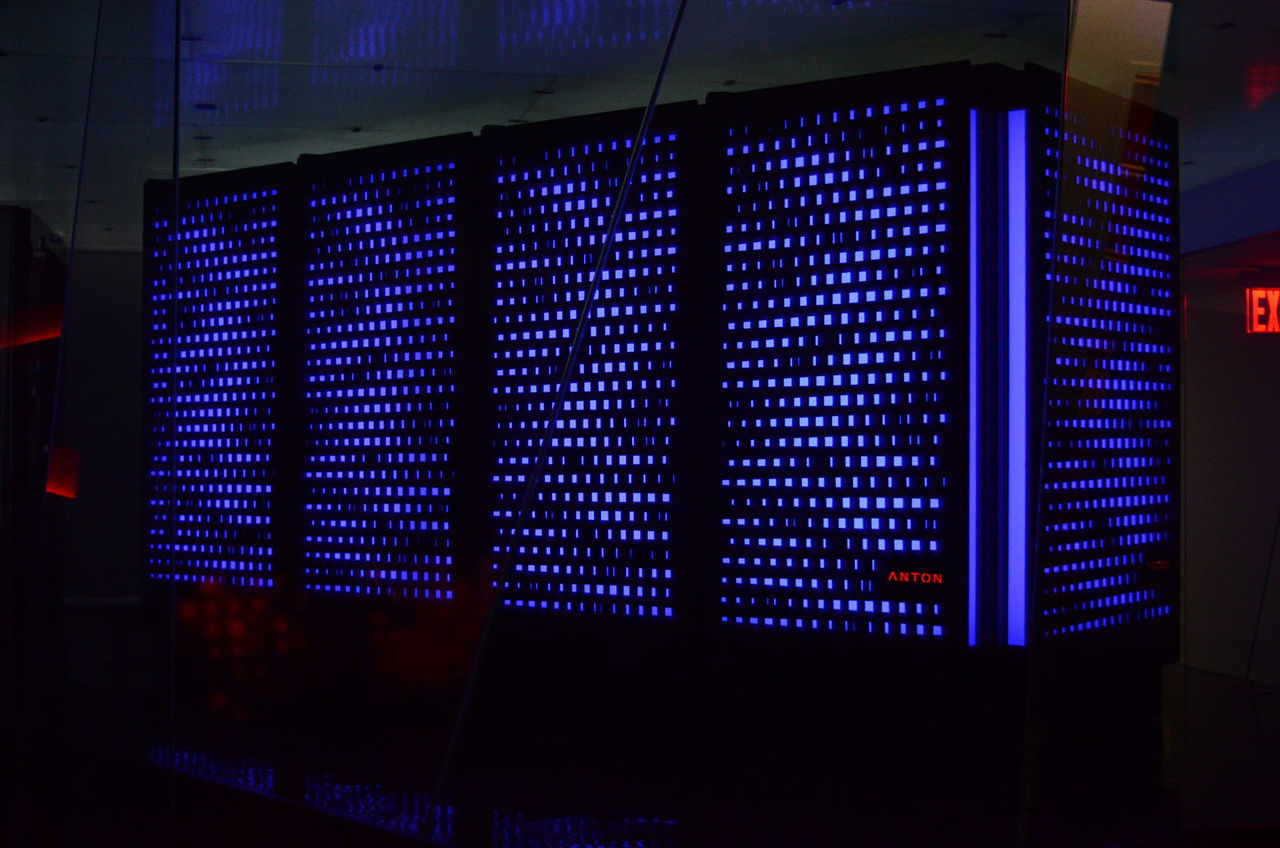
\includegraphics[width=\linewidth]{images/anton.jpg}
  \caption{Anton, a supercomputer built by D.E. Shaw Research specifically for protein folding computations. \cite{Anton} Photo by Matt Simmons}
  \label{fig:anton}
\end{figure}

Even with these speedups, MD simulations are still too slow to be useful purely for structure prediction. For example, a supercomputer purpose-built for protein folding computations, Anton, took around 100 days to simulate a single millisecond of the folding process for a protein comprised of around 1000 atoms \cite{Anton}.

\subsection{Markov State Models for interpreting data from MD simulations}
Despite their suboptimal properties for structure prediction, MD simulations are still valued because they depict the folding process itself. Apart from being theoretically important, this is also of special interest in the study of diseases which are caused by proteins misfolding away from the standard resting conformation; some examples where misfolded proteins are the suspected cause of a disease include Alzheimer's and Huntington's.

To understand folding trajectories of a protein, it is not enough to simulate a single fold of the protein. Instead, a protein's folding process must be simulated many times to derive an understanding of the probability space over the protein's possible conformations. As a result, scientists working on large MD simulations must be able to both gather and comprehend vast amounts of time series data of a protein's probable conformation. I

An excellent tool to guide as well as understand simulation is the \textbf{Markov State Model}.  





\section{Heuristic methods for structure prediction \textit{must} exist}
In nature, proteins regularly attain their resting conformations under a diverse set of initial conditions. The consistency of protein folding suggests that most computations in MD simulations are redundant. Indeed, taking the following abstract view of the folding process leads us to conclude that the protein folding problem \textit{must} be much simpler than the raw physics might suggest.

\subsection{The size of conformational space}
Simulation of protein folding can be equated to drawing a path through the space of possible 3-D conformations of a protein, with each timestep being mapped to a single element of that space. Simulating a full second using femtosecond timesteps would draw a quadrillion samples from this \textbf{conformational space}; though this may seem like a large quantity, a quadrillion samples is in fact minuscule relative to the size of the conformational space itself.

To illustrate the general size of conformational space, note that 3-D conformations are generally parameterized by the set of three dihedral angles, $\psi, \phi, \omega$, between each conjoined pair of atoms. $\omega$ is usually uniformly restricted to be in the set $\{180^\circ, 0^\circ\}$ since peptide bonds are almost always planar, but $\psi$ and $\phi$ can take on all possible degrees. If we discretized the angles into 3 states each, a chain of 100 amino acids would thus have $3^198$ possible conformations for the 99 bonds between each conjoined pair of residues \cite{levinthal}. Even if all physically impossible conformations were removed, the number of conformations would still be on roughly this same order.

\subsection{Levinthal's Paradox and Anfinsen's Dogma}
With these numbers, it can be seen that even if a unique conformation was sampled each femtosecond since the beginning of time, the aforementioned 100-chain protein still would not have seen nearly all the possible conformations. This insight is known as \textbf{Levinthal's paradox}, and it shows that the process of protein folding cannot possibly be random. The sheer size of conformational space, combined with the empirical stability of the protein folds under the tremendously different initial conditions experienced in nature everyday shows that the protein folding process is almost surely determined. Therefore, most of the information obtained from protein folding simulations is irrelevant with respect to determining the resting conformation. A variant of this belief is known as \textbf{Anfinsen's Dogma}, which hypothesizes that the resting conformation is almost always fully determined by the amino acid sequence \cite{anfinsen}.

\newpage 
\vfill
\begin{figure}[!h]
  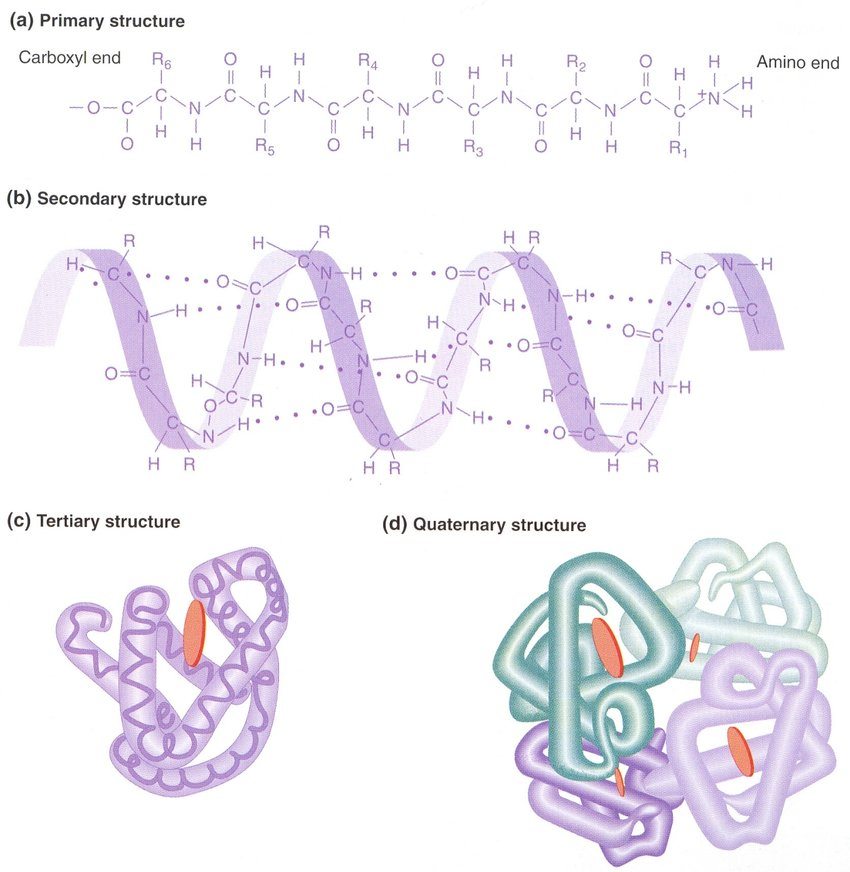
\includegraphics[width=\linewidth]{images/protein_structure.png}
  \caption{An illustration of the different levels of protein structure. Graphic from \cite{genetic_analysis}}
  \label{fig:proteinStructure}
\end{figure}

\section{The hierarchical structure of protein folds, as seen in data}
The \textbf{physics-based} view of protein folding is too granular to yield insights into the structure of protein folds. An approach that has seen more success is working directly with known protein structures to extrapolate to unknown structures. This \textbf{knowledge-based} approach assumes that protein structure forms an emergent system which can be studied in its own right, much like chemistry can be seen as an emergent property of the laws of physics.

The vocabulary of protein structures is hierarchically divided into four tiers: \textit{primary, secondary, tertiary}, and \textit{quaternary}. An illustration of the different structures given by \autoref{fig:proteinStructure}. We go through each in turn.

\paragraph{Primary} Primary structure simply denotes the amino acid sequence comprising the protein. The alphabet of primary structure is composed of the amino acids themselves. Of roughly 500 naturally occurring amino acids, only 22 are used to construct proteins. Of these 22, only 20 are found in genetic code, and the other 2 are inserted after the protein's initial creation \cite{20proteins}.

Sequences of 30 amino acids or less are generally considered peptides. Most proteins are comprised of several hundred amino acid residues, though the largest can go have as many as 27000 residues. Naively, this places the space of primary structure at roughly $20^{27000}$, an incomprehensible number. Of course, just as a single protein samples a minuscule amount of its possible conformations, the sum total of natural proteins only sample a minuscule amount of sequence space. A simple estimate by \cite{sequenceExploration} places the number of sampled protein sequences seen at some point in history at roughly $4 * 10^{21}$, and argues this is around the true number of naturally viable proteins.

\paragraph{Secondary}

\paragraph{Tertiary}

\paragraph{Quaternary}

\section{Hidden Markov Models for Mining Primary Structure Data}
Though primary structures are the rawest form of protein data, they are also the most numerous available to knowledge-based techniques. Frequently, primary structures obtained from genome sequencing are the only evidence a protein exists. As of November 2019, UniProt, a leading database of biological sequences, contains 181787788 sequences, or roughly $1.8 * 10^8$ \cite{uniprot}. A breakdown is given in \autoref{tab:uniprot}. 

\begin{table}[h!]
    \centering
       \begin{tabular}{|c||c||c|}
        \hline
        \hline
        Protein existence & Entries & Percent \\ \hline
        Evidence at protein level & 151242 & 0.08\% \\ \hline
        Evidence at transcript level & 1297981 & 0.71\% \\ \hline
        Inferred from homology & 45460655 & 25.01\% \\ \hline
        Predicted & 134877910 & 74.20\% \\ \hline
        \end{tabular}
    \caption{Breakdown of entries in the UniProt database}
    \label{tab:uniprot}
\end{table}

\subsection{Error-correcting codes for shotgun sequencing of a genome}


\subsection{HMMs for Multiple Sequence Alignment}
Knowing the primary structure of the protein does not give us anything near a deterministic calculation of the resting conformation a la Anfinsen's Dogma, but it does yield some information. In particular, if we have sequenced many organisms, studying the differences in how common proteins are coded yields information on which amino acids in the sequence are mutating together or \textbf{co-evolving}. Frequently, amino acids which co-evolve are physically close in the resting conformation. 


The space of naturally occurring protein sequences can be estimated by sequencing the genomic data of various organisms. 

extrapolate to the structures of unknown proteins, 

The number of known folds is low. Closely related sequences tend to be close in structure. We can leverage data to get starting "templates" instead of recomputing everything from scratch.


\section{Fragment Assembly for Assembling Secondary structure}
Can be classified into $\alpha$-helices and $\beta$-sheets.

Fragment libraries

\paragraph{Threading}

\section{Tertiary structure}
Only about 1000 general forms, but the number of angles, contacts, etc. are legion

\paragraph{Imaged structures deposited in the Protein Data Bank}

\paragraph{Folding trajectories from molecular dynamics simulations}

\paragraph{Guesses from existing folding software}

\section{Knowledge-based energy functions derived from data of known structures}


\printbibliography

\end{document}
